\documentclass[11pt]{article}
\usepackage[utf8]{inputenc}
\usepackage[T1]{fontenc}
\usepackage{mathpazo}
\usepackage{xcolor}
\usepackage{graphicx}
\usepackage{dblfloatfix}
\usepackage{amsmath}
\PassOptionsToPackage{hyphens}{url}\usepackage{hyperref}
\usepackage{hyperref}
\usepackage{url}
\graphicspath{{./images/}}

\begin{document}
	
	\begin{titlepage}
		\newcommand{\HRule}{\rule{\linewidth}{0.5mm}}
		
		\centering
		
		\textsc{\LARGE OMNO AI}\\[0.5cm]
		
		\textsc{\Large Onward and Upwards}\\[1.5cm]
		
		\HRule\\[0.4cm]
		
		{\huge\bfseries Emotion Detection}\\[0.4cm]
		
		\HRule\\[1.5cm]
		
		\begin{minipage}{0.4\textwidth}
			\begin{flushleft}
				\large
				\textit{Author:}\\
				Ibtihaj Tahir
			\end{flushleft}
		\end{minipage}
		~
		\begin{minipage}{0.4\textwidth}
			\begin{flushright}
				\large
				\textit{Team Leads:}\\
				Hussam Habib\\
				Kaleem Khan
			\end{flushright}
		\end{minipage}
		
		\vfill\vfill\vfill
		
		{\large\today}
		
		\vfill\vfill\vfill
		
\includegraphics[width=0.5\textwidth]{logo.png}\\[1cm]
		
	\end{titlepage}

	\tableofcontents
	\newpage
	
	\section{Problem Statement}
		Facial expressions are a very powerful way of communication without words. By just looking at someone's expression, we can tell that weather the person is sad, happy or angry and all. A set of muscles are present on human's face that adjust there self with respect to the mood and hence form facial expressions. We, as humans can easily tell the mood by looking at the other person's expressions but for a machine to recognize it is not that simple.
		\newline
		\newline
		Goal is to device a method by using the modern Deep Learning approaches to recognize human's face expressions.
		\newline
		\newline
		\newline
		\newline
		\begin{figure*}[ht]
			\centering
			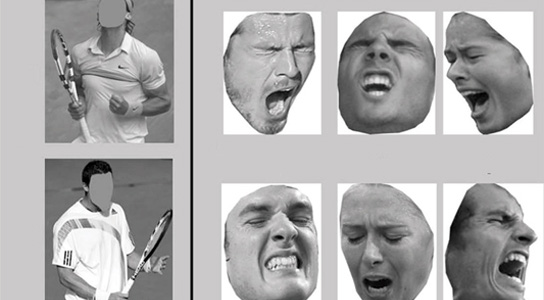
\includegraphics[width=0.5\textwidth]{problem_st}
		\end{figure*}
		
		\newpage
		
	\section{Datasets}
	\subsection{FER2013 \cite{carrier2013fer}}
	The data consists of 48x48 pixel gray-scale images of faces. The faces have been automatically registered so that the face is more or less centered and occupies about the same amount of space in each image. The task is to categorize each face based on the emotion shown in the facial expression in to one of seven categories (0=Angry, 1=Disgust, 2=Fear, 3=Happy, 4=Sad, 5=Surprise, 6=Neutral).
	\newline
	\newline
	The cvs contains two columns, "emotion" and "pixels". The "emotion" column contains a numeric code ranging from 0 to 6, inclusive, for the emotion that is present in the image. The "pixels" column contains a string surrounded in quotes for each image. The contents of this string a space-separated pixel values in row major order. The dataset consists of 35,887 images.
	\newline
	\newline
	The dataset can be obtained from
	\newline
	\def\UrlFont{\bfseries}
	\url{https://www.kaggle.com/c/challenges-in-representation-learning-facial-expression-recognition-challenge/data}
	\newline
	\newline
	\newline
	\newline
	\begin{figure*}[ht]
		\centering
		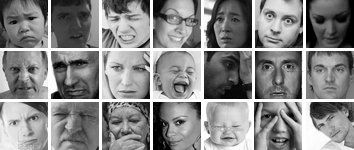
\includegraphics[width=0.5\textwidth]{fer2013_images}
		\caption{Samples from FER2013}
	\end{figure*}
	
	\newpage
	
	\subsection{CK+ \cite{lucey2010extended}}
	\textbf{The Images} (cohn-kanade-images.zip) -  there are 593 sequences across 123 subjects which are FACS coded at the peak frame. All sequences are from the neutral face to the peak expression.
	\newline
	\newline
	\textbf{The Landmarks} (Landmarks.zip) - All sequences are AAM tracked with 68points landmarks for each image.
	\newline
	\newline
	\textbf{The FACS coded files} (FACS\_labels.zip) - for each sequence (593) there is only 1 FACS file, which is the last frame (the peak frame). Each line of the file corresponds to a specific AU and then the intensity. An example is given below.
	\newline
	\newline
	\textbf{The Emotion coded files} (Emotion\_labels.zip) - ONLY 327 of the 593 sequences have emotion sequences. This is because these are the only ones the fit the prototypic definition. Like the FACS files, there is only 1 Emotion file for each sequence which is the last frame (the peak frame). There should be only one entry and the number will range from 0-7 (i.e. 0=neutral, 1=anger, 2=contempt, 3=disgust, 4=fear, 5=happy, 6=sadness, 7=surprise). N.B there is only 327 files- IF THERE IS NO FILE IT MEANS THAT THERE IS NO EMOTION LABEL (sorry to be explicit but this will avoid confusion).
	\newline
	\newline
	The dataset can be obtained from
	\newline
	\def\UrlFont{\bfseries}
	\url{http://www.consortium.ri.cmu.edu/ckagree/}
	\begin{figure*}[ht]
		\centering
		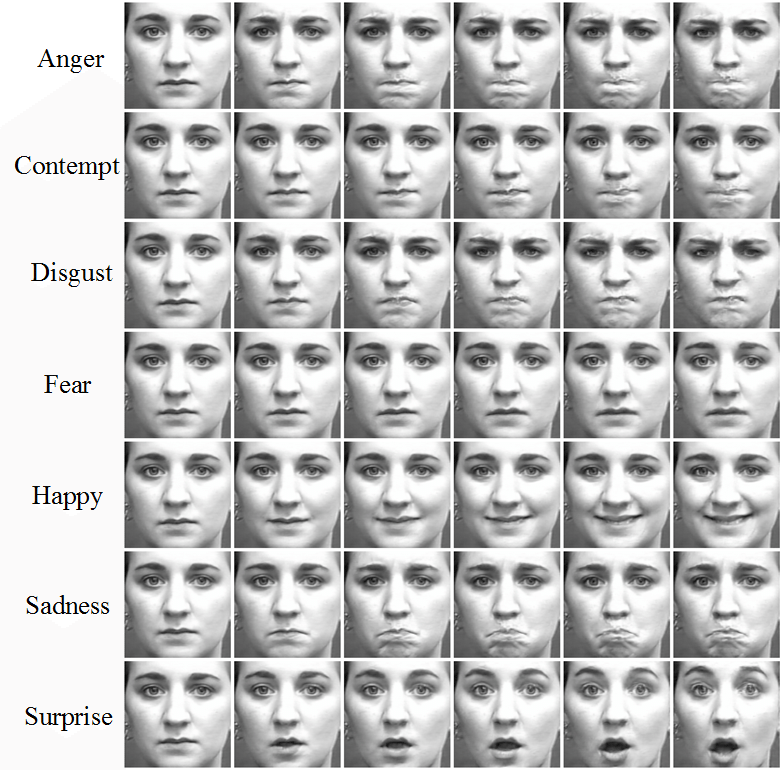
\includegraphics[width=0.4\textwidth]{ck+_images}
		\caption{Samples from CK+}
	\end{figure*}
	\newpage
	
	\section{Deep Learning Models}
	\subsection{VGG16 \cite{simonyan2014very}}
	\begin{figure*}[ht]
		\centering
		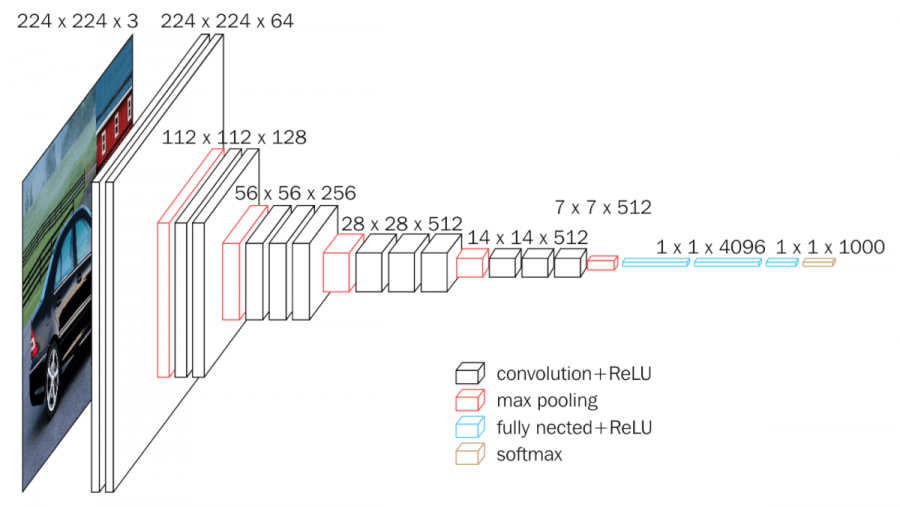
\includegraphics[width=0.6\textwidth]{vgg16_arch}
		\caption{VGG16}
	\end{figure*}
    VGG16 is a Convolutional Neural Network model proposed by K. Simonyan and A. Zisserman from the University of Oxford. The model achieves 92.7\% top\-5 test accuracy in ImageNet, which is a dataset of over 14 million images belonging to 1000 classes. It was one of the famous model submitted to \href{http://www.image-net.org/challenges/LSVRC/2014/results}{ILSVRC-2014}. It makes the improvement over AlexNet by replacing large kernel\-sized filters with multiple 3x3 kernel\-sized filters one after another.
    
    \subsection{Resnet50 \cite{he2016deep}}
    \begin{figure*}[ht]
    	\centering
    	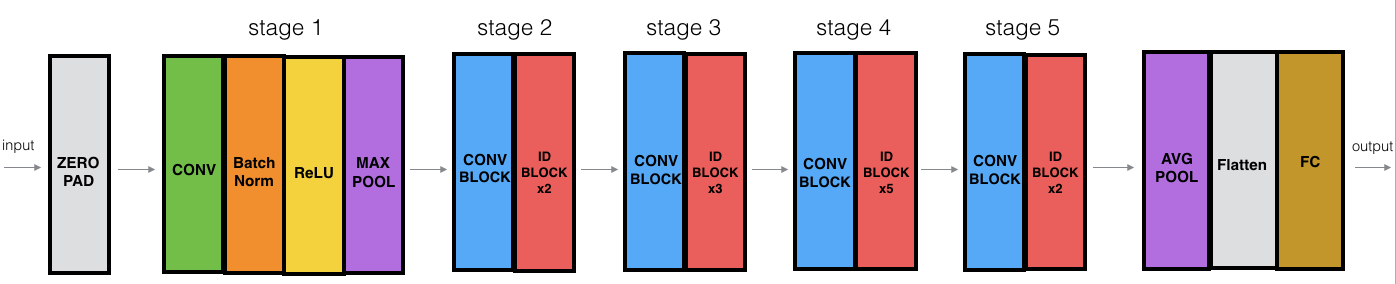
\includegraphics[width=0.8\textwidth]{resnet50_arch}
    	\caption{Resnet50}
    \end{figure*}
    Residual Networks is a classic neural network used as a backbone for many computer vision tasks. This model was the winner of ImageNet challenge in 2015. The fundamental breakthrough with ResNet was it allowed us to train extremely deep neural networks with 150+layers successfully. Prior to ResNet training very deep neural networks was difficult due to the problem of vanishing gradients.
    AlexNet, the winner of ImageNet 2012 and the model that apparently kick started the focus on deep learning had only 8 convolutional layers, the VGG network had 19 and Inception or GoogleNet had 22 layers and ResNet 152 had 152 layers.
    \newline
    \newline 
    The ResNet-50 model consists of 5 stages each with a convolution and Identity block. Each convolution block has 3 convolution layers and each identity block also has 3 convolution layers. The ResNet-50 has over 23 million trainable parameters.
    
    \subsection{Inception V3 \cite{szegedy2016rethinking}}
    \begin{figure*}[ht]
    	\centering
    	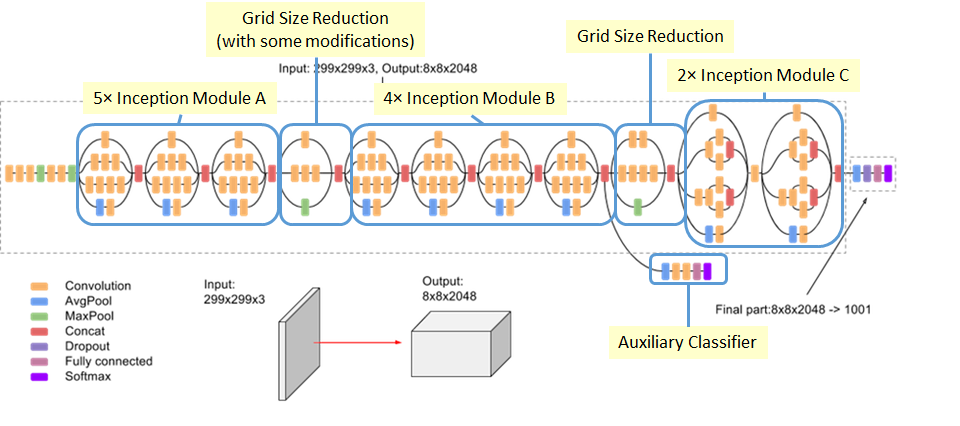
\includegraphics[width=0.8\textwidth]{inceptionv3_arch}
    	\caption{InceptionV3}
    \end{figure*}
Inception v3 is a widely-used image recognition model that has been shown to attain greater than 78.1\% accuracy on the ImageNet dataset. The model itself is made up of symmetric and asymmetric building blocks, including convolutions, average pooling, max pooling, concats, dropouts, and fully connected layers. Batchnorm is used extensively throughout the model and applied to activation inputs. Loss is computed via Softmax. 
\newpage

	\subsection{Inception-Resnet-V2 \cite{szegedy2017inception}}
	\begin{figure*}[ht]
		\centering
		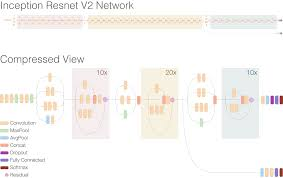
\includegraphics[width=0.8\textwidth]{inceptionresnet_arch}
		\caption{Inception\_Resnet\_V2}
	\end{figure*}
	
	Very deep convolutional networks have been central to
	the largest advances in image recognition performance in
	recent years. One example is the Inception architecture that
	has been shown to achieve very good performance at relatively low computational cost. Recently, the introduction
	of residual connections in conjunction with a more traditional architecture has yielded state-of-the-art performance
	in the 2015 ILSVRC challenge; its performance was similar
	to the latest generation Inception-v3 network. This raises
	the question of whether there are any benefit in combining
	the Inception architecture with residual connections. Here
	we give clear empirical evidence that training with residual
	connections accelerates the training of Inception networks
	significantly. There is also some evidence of residual Inception networks outperforming similarly expensive Inception
	networks without residual connections by a thin margin. We
	also present several new streamlined architectures for both
	residual and non-residual Inception networks. These variations improve the single-frame recognition performance on
	the ILSVRC 2012 classification task significantly. We further demonstrate how proper activation scaling stabilizes
	the training of very wide residual Inception networks. With
	an ensemble of three residual and one Inception-v4, we
	achieve 3.08\% top-5 error on the test set of the ImageNet
	classification (CLS) challenge.
	\newpage
	
	\subsection{DeXpression \cite{burkert2015dexpression}}
	\begin{figure*}[ht]
		\centering
		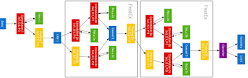
\includegraphics[width=0.5\textwidth]{deXpression_arch}
		\caption{DeXpression}
	\end{figure*}
The proposed deep Convolutional Neural Network architecture consists of four parts.
The first part automatically preprocesses the data. This
begins with Convolution 1, which applies 64 different
filters. The next layer is Pooling 1, which down-samples
the images and then they are normalized by LRN 1. The
next steps are the two FeatEx (Parallel Feature Extraction
Block) blocks. They are the core of the proposed architecture. The features extracted by theses blocks are
forwarded to a fully connected layer, which uses them
to classify the input into the different emotions.
The described architecture is compact, which makes it
not only fast to train, but also suitable for real-time
applications. This is also important as the network was
built with resource usage in mind. \newline The key structure in the architecture is the
Parallel Feature Extraction Block (FeatEx). It is inspired
by the success of GoogleNet. The block consists of
Convolutional, Pooling, and ReLU Layers. The first
Convolutional layer in FeatEx reduces the dimension
since it convolves with a filter of size 1 x 1. It is
enhanced by a ReLU layer, which creates the desired
sparseness. The output is then convolved with a filter
of size 3 x 3. In the parallel path a Max Pooling layer
is used to reduce information before applying a CNN
of size 1 x 1. This application of differently sized filters
reflects the various scales at which faces can appear.
The paths are concatenated for a more diverse
representation of the input. Using this block twice
yields good results.
	
	\newpage
	\section{Implementation}
	Both the dataset (CK+ and fer2013) are used to train all the above mentioned models. The following hyper-parameters were used.
	\begin{itemize}
		\item Random Seed is set to 7 for reproduction of the results
		\item A train-test split of 5\%
		\item For CK+, batch size is set to be 8 for train and 4 for test
		\item For Fer2013, batch size is set to be 32 for train and 16 for test
		\item \textbf{'categorical\_crossentropy'} loss is used to train all the algorithms
		\item \textbf{'Adam'} optimizer is used to train all the algorithms
		\item 200 epochs
		\item 100 step-size
		\item 100 validation-step 
		
	\end{itemize} 
	\textbf{Note: }These parameters can be adjusted to achieve different results.
	\newline
	\newline
	Implementation can be found at
	\newline
	\url{https://github.com/IT-OMNOAI/Smart-Gandola}

	\newpage

	\section{Results}
	\subsection{CK+}
	\begin{itemize}
		\item \textbf{VGG16}
		\begin{figure*}[ht]
			\centering
			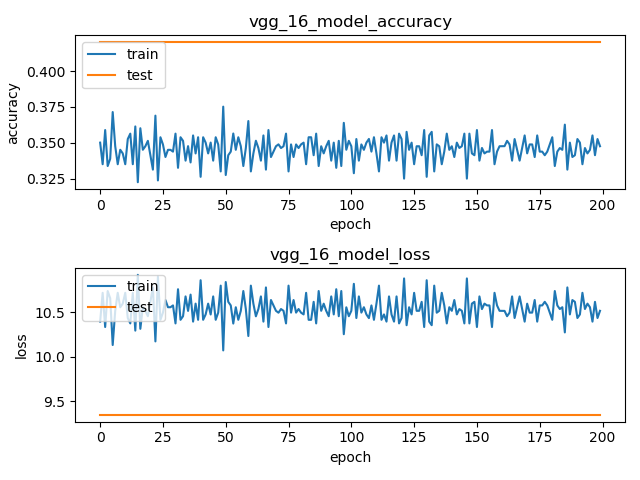
\includegraphics[width=0.6\textwidth]{vgg16_res}
			\caption{VGG16 on CK+}
		\end{figure*}

		\item \textbf{Resnet50}
		\begin{figure*}[ht]
			\centering
			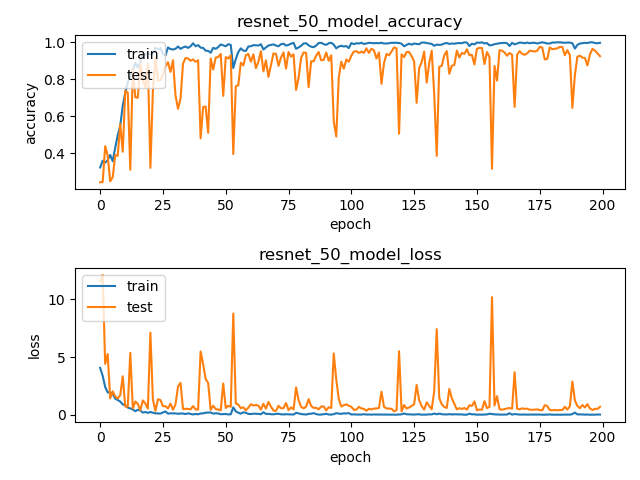
\includegraphics[width=0.6\textwidth]{resnet50_res}
			\caption{Resnet50 on CK+}
		\end{figure*}
	\newpage
		
		\item \textbf{InceptionV3}
		\begin{figure*}[ht]
			\centering
			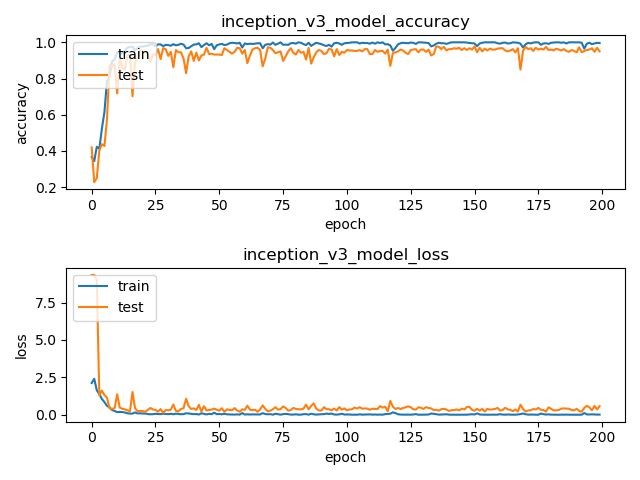
\includegraphics[width=0.6\textwidth]{inceptionV3_res}
			\caption{InceptionV3 on CK+}
		\end{figure*}
	
		\item \textbf{InceptionResnetV2}
		\begin{figure*}[ht]
			\centering
			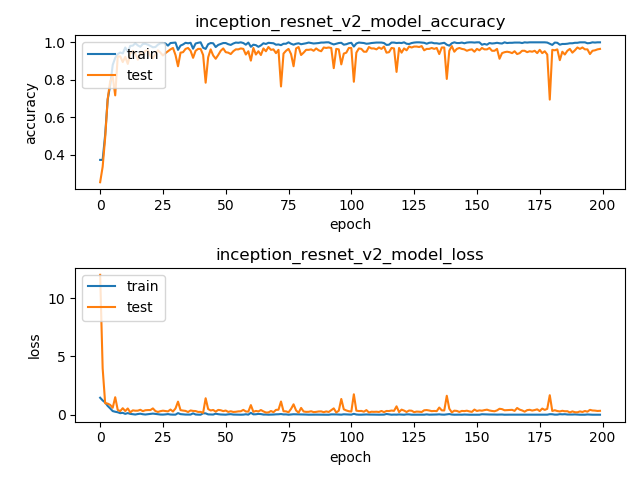
\includegraphics[width=0.6\textwidth]{inceptionResnetV2_res}
			\caption{InceptionResnetV2 on CK+}
		\end{figure*}
				
		\newpage
			
		\item \textbf{DeXpression}
		\begin{figure*}[ht]
			\centering
			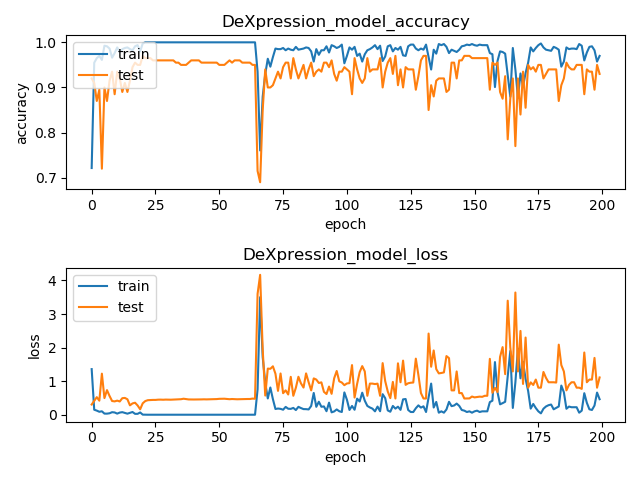
\includegraphics[width=0.6\textwidth]{DeXpression_CK+_res}
			\caption{DeXpression on CK+}
		\end{figure*}
		
	\end{itemize}

	\subsection{FER2013}
	\begin{itemize}
		\item \textbf{DeXpression}
		\begin{figure*}[ht]
			\centering
			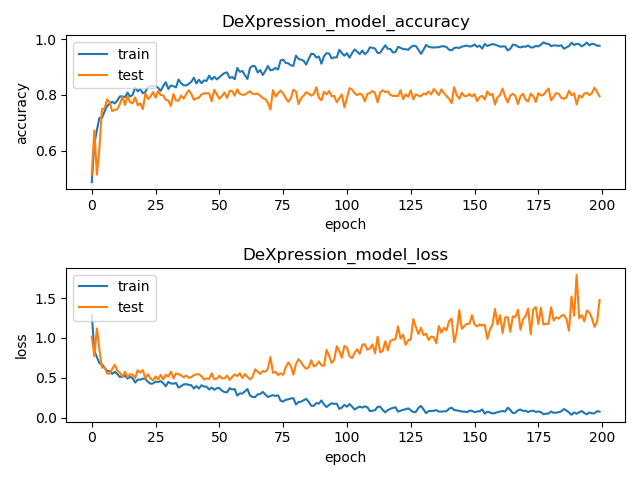
\includegraphics[width=0.6\textwidth]{DeXpression_FER_res}
			\caption{DeXpression on FER2013}
		\end{figure*}
	\end{itemize}

	\textbf{InceptionV3} trained on \textbf{CK+} and \textbf{DeXpression} trained on \textbf{FER2013} has been tested and have proved great accuracy on finding the right expression. The stability of models can be seen with the training results of the model. 
	
	
	\newpage
	
\bibliography{papers} 
\bibliographystyle{ieeetr}

\end{document}
